\section{B1}
\label{sec:B1}

Plusieurs approches techniques existent dans le domaine du streaming de données. Nous allons travailler avec des tweets mais il est possible d'appliquer toutes ces techniques dans d'autres domaines.\\

\subsection{Envoi des données pour analyse}
\label{sub:Envoi des données pour analyse}

  Tout d'abord, la première solution technique existante est l'envoi des données au fur et à mesure de leur arrivée. Dans notre cas: Twitter envoie chaque tweets au fur et à mesure de leur émission sur ce que l'on appelle un \textit{endpoint}. L'envoi de chaque tweet peut-être effectué suivant plusieurs protocoles différents comme HTTP pour le plus connu ou encore par un protocole créé spécialement pour l'application via de simples sockets réseaux.\\

  \paragraph{Avantage de la solution}
  \label{par:Avantage de la solution}
  Le principal avantage de cette technique est la rapidité du transfert de l'information. Les tweets sont traité à la même vitesse que leur création et l'information créé est donc réellement en temps réel (sans compter les temps de transfert de l'information de Twitter à notre programme de traitement ni le temps de traitement).

  \paragraph{Inconvénients de la solution}
  \label{par:Inconvénients de la solution}
  Cet avantage peut se transformer en inconvénient si l'\textit{endpoint} n'est pas capable d'absorber l'information assez rapidement. Au vu de la quantité de tweets envoyés sur Twitter, il est très compliqué de concevoir un système capable de réagir à la masse de données reçues. Dans le cas où le système ne permet plus de traiter les tweets, il cesse de répondre et les tweets envoyés par Twitter sont donc perdus.\\

  \paragraph{Outils pratiques}
  \label{par:Outils pratiques}
  Twitter ne propose pas actuellement de sytème d'\textit{endpoint}. Ce choix est facilement compréhensible au vu des inconvénients évoqués dans le paragraphe précédent. Il est par contre possible de mettre en place ce genre d'architecture pour des volumes de données moindres comme par exemple lors de l'exécution de l'envoi d'un message sur \href{https://slack.com/}{Slack} ou IRC (plateformes de messagerie instantanée). L'\textit{endpoint} peut dans ce cas exécuter des programmes spécifiques en fonction du message reçu.

\subsection{Utilisation de queues de messages}
\label{sub:Utilisation de queues de messages}

  Afin de résoudre le problème de la masse de tweets reçue par l'\textit{endpoint}, il est possible d'utiliser des queues de messages. Ces queues de messages n'ont pas vocations à traiter les données mais seulement les stocker en attendant la consommation.\\

  Avec cette solution technique, l'action de traitement ne reçoit plus les tweets en temps réel mais peut venir les récupérer dès qu'elle en a besoin dans la queue de messages. Nous ne sommes plus dans une situation de réception mais bien de récupération de l'information.\\

  \paragraph{Avantages de la solution}
  \label{par:Avantages de la solution}
  Cette solution permet de mieux réguler le flux de tweets car la queue n'a plus de problèmes pour absorber la masse de tweets envoyés car elle ne traite pas l'information. Le programme de traitement quant-à-lui peut récupérer l'information dès qu'il en a besoin. Le traitement est donc mieux réparti entre les périodes avec un fort volume de tweets (ou le traitement va prendre du retard) et les périodes de faible volume de tweets (ou le traitement va prendre de l'avance).

  \paragraph{Inconvénients de la solution}
  \label{par:Inconvénients de la solution}
  L'utilisation de la queue est tout de même limitée en terme d'espace de stockage. En effet, si le retard accumulé par le traitement devient trop important et qu'il devient impossible de stocker les tweets dans la queue (par manque de RAM pour une queue en mémoire vive ou d'espace disque pour une queue persistée sur disque), il est nécessaire de supprimer des anciens tweets ou de refuser des nouveaux tweets. Une information est donc perdue.

  \paragraph{Outils pratiques}
  \label{par:Outils pratiques}
  De nombreux outils de queues de messages existent. Il est possible d'utiliser Apache Flume ou Apache Kafka en auto-hébergé. Il est également possible de profiter de l'offre cloud d'AWS nommé Amazon Kinesis. Ces trois outils fonctionnent de la même manière: une source de données (Twitter dans notre cas), un tuyau stockant les tweets et un puit (notre programme de traitement).\\

  Ces trois outils sont des queues de messages distribuées. Cela signifie que ces programmes peuvent fonctionner sur plusieurs machines physiques ou virtuelles. Concernant Amazon Kinesis, l'architecture fonctionne par \textit{shards} qui sont des tuyaux distribués. Il faut donc gérer plusieurs consommateurs de la queue différents. Ces consommateurs ne vont pas accéder à toute l'information mais seulement une partie des tweets. Dans notre cas, les tweets sont des événements totalement indépendants cette multitude de consommateurs est donc sans importance. Dans le cas où les événements mis en queue pourrait être liés entre eux, deux solutions sont possibles: agréger les messages avant l'insertion dans la queue ou choisir une clé de partitionnement permettant d'insérer les messages liés dans le même tuyau et ainsi les traiter avec le même consommateur.

\subsection{Traitement des données de manière distribuée}
\label{sub:Traitement des données de manière distribuée}

  Nos queues de messages sont distribuées pour permettre de meilleures performances et une facilité dans l'amélioration de la puissance de stockage de la queue. Il est très intéressant également de travailler sur un programme de traitement des données distribué. En effet, il serait donc possible d'améliorer les perforances et les temps de calcul de notre programme en ajoutant de nouvelles machines.\\

  Pour permettre l'utilisation de machines distribuées, il est nécessaire que les données ainsi que l'algorithme soient distribués. Le pattern le plus réputé dans le domaine est celui du Map / Reduce (figure \ref{mapreduce}). Dans ce pattern, deux opérations sont définies: les opérations de \textit{mapping} qui s'exécutent en local sur chaque machine et permettre d'exploiter toute la puissance du distribué, et les opérations de type \textit{reduce} qui permette d'aggréger les résultats de toutes les machines sur la machine principale afin de les sauvegarder ou les exploiter. Cette dernière opération n'étant pas distribué, il faut faire particulièrement attention aux volumes de données remontés par les opérations de type \textit{reduce} afin de prévenir tout problème au niveau de la machine principale.

  \begin{figure}
    \centering
    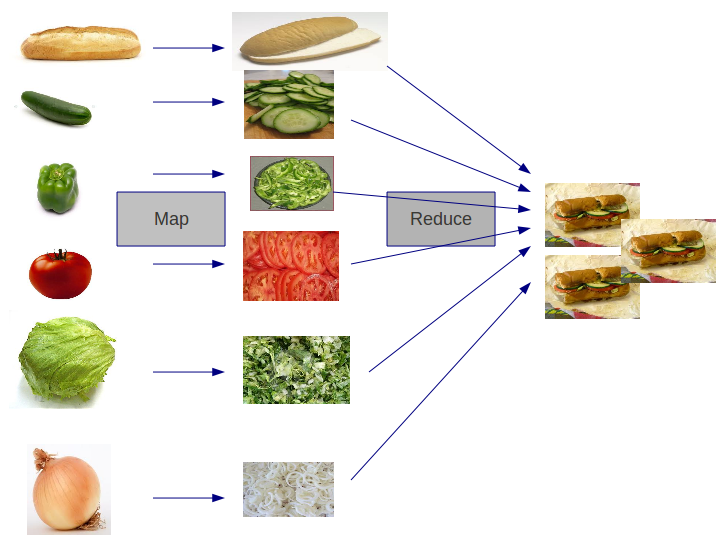
\includegraphics[width=0.8\textwidth]{images/mapreduce.png}
    \caption{Concept Map / Reduce expliqué à l'aide d'un sandwich.}
    \label{mapreduce}
  \end{figure}


\section{B2}
\label{sec:B2}
  \subsection{Spark Streaming}
  Afin de garantir un traitement distribué, il est possible d'utiliser le framework Apache Spark et plus précisément Spark Streaming pour traiter le flux de messages en temps réel ou de façon continue. Cet outil possède une bibliothèque (\emph{spark-streaming-twitter\_2.10}) permettant de communiquer directement avec l'API de Twitter. Il n'y a aucune restriction pour l'utilisation d'Apache Spark et sa bibliothèque, car ce sont des logiciels \emph{Open Source}.

  \subsection{Hadoop avec Flume}
  \label{sub:Hadoop avec Flume}
  D'autres solutions existent pour effectuer des calculs distribués comme le framework Apache Hadoop. Il est également possible de mettre en place notre propre système de queues de messages avec Apache Flume. Il existe une source de données pour Apache Flume correspondant à l'API Twitter développée par Cloudera. Ces deux technologies sont \emph{Open Source} et ne nécessitent donc aucune license.

  \subsection{API HTTP Twitter Streaming}
  Il existe une solution non distribuée qui consiste à consommer le flux Twitter sous forme d'API HTTP. Twitter propose de télécharger un fichier à distance d'une taille infinie contenant tous les tweets. Plusieurs restrictions s'imposent mais il est possible de gérer ce téléchargement infini grâce à des bibliothèques de client HTTP dans n'importe quel langage. Le client doit simplement pouvoir gérer le traitement en temps réel du résultat de la requête HTTP.

\section{B3}
\label{sec:B3}
  \subsection{Spark Streaming}
    Afin de gérer le flux continu de données, Spark streaming va discrétiser le flux en \emph{batch}, c'est à dire en tranches d'informations. Ensuite, Spark va pouvoir effectuer les traitements ou calculs sur chacun de ces \emph{batch} de données de manière individuelle. La figure~\ref{streaming_flow} illustre ce découpage de flux de données. \\

  \begin{figure}
    \centering
    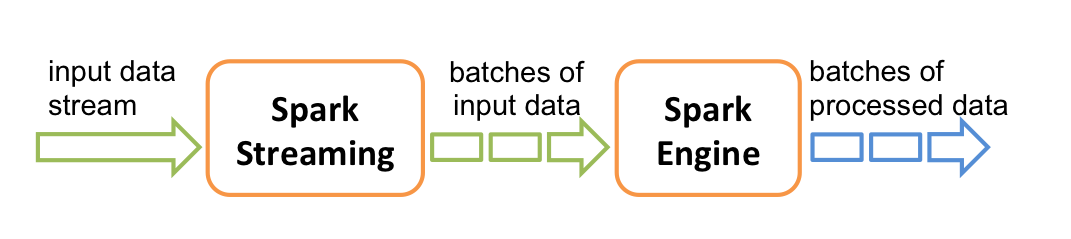
\includegraphics[width=0.8\textwidth]{images/streaming-flow.png}
    \caption{Découpage du flux de données par Spark Streaming}
    \label{streaming_flow}
  \end{figure}

  Le flux n'est donc plus continue mais représenté par une couche d'abstraction appelée \emph{Discretized Stream} ou \emph{Dstream}. Chaque \emph{batch} peut être traité de manière indépendante et donc parallélisé. Par exemple, si l'on cherche à récupérer les mots d'un flux de lignes de texte, Spark va créer des \emph{batch} avec un certain nombre de lignes qui seront ensuite analysées individuellement pour obtenir les mots qui composent ces lignes de texte. La figure~\ref{streaming_dstream_get_word} présente cet exemple. Un grand nombre d'opérations peuvent être réalisés sur ces \emph{batch} de données, comme par exemple \emph{map}, \emph{reduce}, \emph{filter}, \emph{union}, \emph{count}… \\

  \begin{figure}
    \centering
    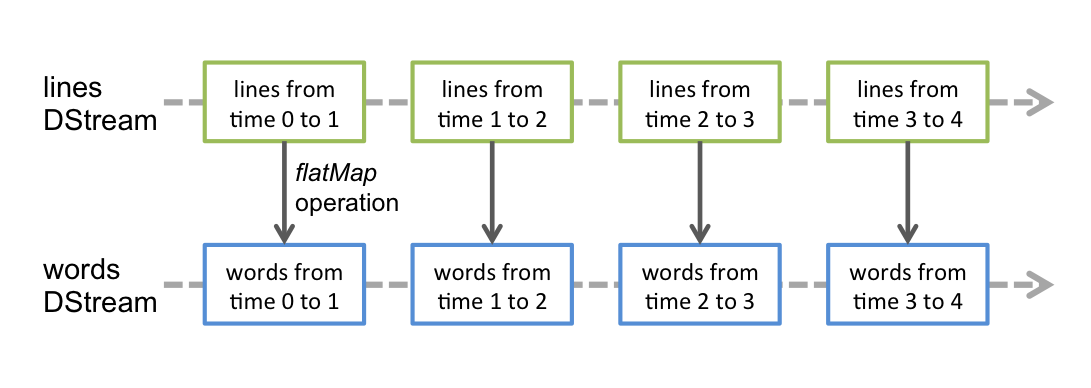
\includegraphics[width=0.8\textwidth]{images/streaming-dstream-ops.png}
    \caption{Exemple de récupération de mots par \emph{batch}}
    \label{streaming_dstream_get_word}
  \end{figure}

  Le flux étant discrétiser, Spark Streaming fournit des paramètres afin de régler la taille de la fenêtre de discrétisation, ainsi que l'intervalle entre deux lancements de calculs. Sur la figure~\ref{principe_de_fenetre_spark_streaming}, nous pouvons observer une taille de fenêtre d'une unité de temps entre chaque \emph{batch} (en vert), une taille de fenêtre de discrétisation regroupant les \emph{batch} de trois (en jaune) et un intervalle de deux entre chaque lancements de calculs sur les fenêtres de discrétisation (en rouge).

  \begin{figure}
    \centering
    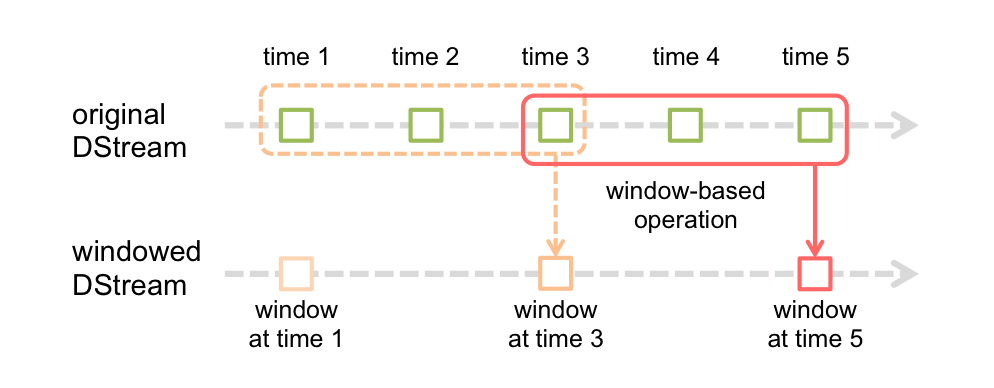
\includegraphics[width=0.8\textwidth]{images/streaming-dstream-window.png}
    \caption{Principe de fenêtrage}
    \label{principe_de_fenetre_spark_streaming}
  \end{figure}

  \subsection{API HTTP Twitter Streaming }
  \label{sub:API HTTP Twitter Streaming}
  Cette seconde solution possède une architecture beaucoup plus simple car elle n'est pas distribuée.


\section{B4}
\label{sec:B4}


\section{B5}
\label{sec:B5}
  La figure~\ref{WBS} représente notre \emph{Work Breakdown Structure} pour nos deux prototypes.

  \begin{figure}
    \centering
    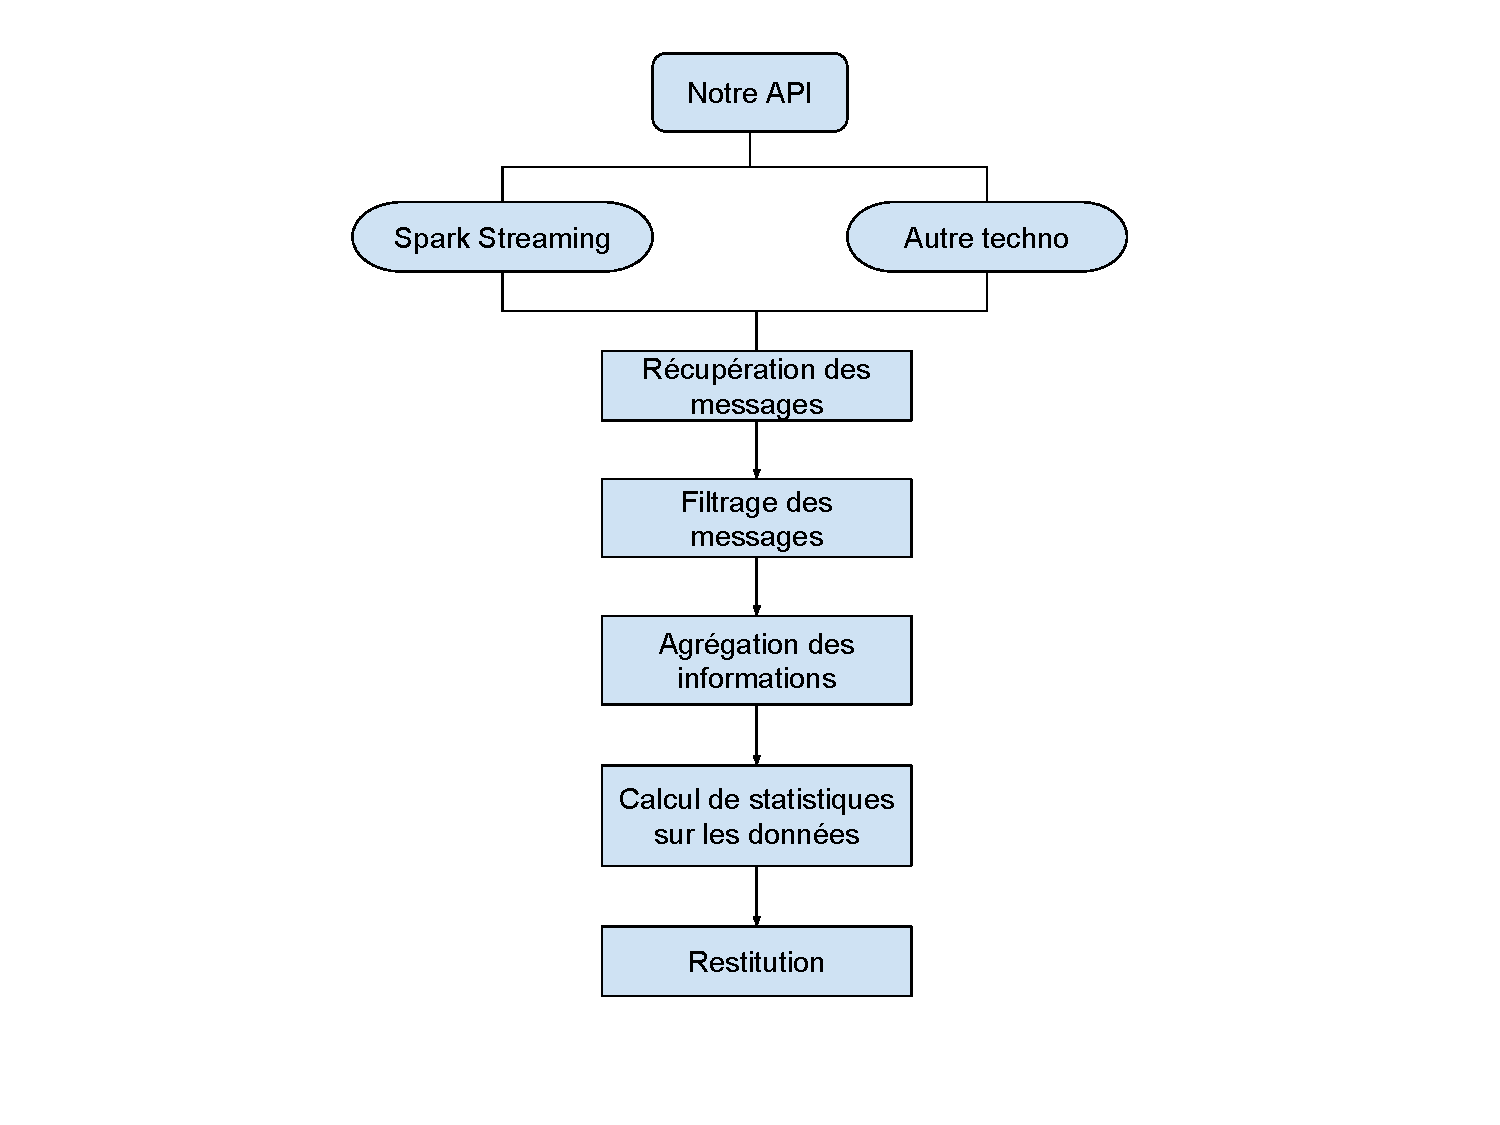
\includegraphics[width=1\textwidth]{images/WBS.pdf}
    \caption{WBF des prototypes}
    \label{WBS}
  \end{figure}
